\documentclass[../DefinizioneDiProdotto.tex]{subfiles}

\begin{document}

\section{Architettura applicazione}

	\subsection{Architettura ad alto livello}
		L'architettura dell'applicazione rispecchia il pattern architetturale a livelli presentando quattro livelli:
		\begin{description}
			\item[Presentation layer:] contiene le componenti dell'interfaccia grafica utente passiva e le componenti facenti parte dell'interfaccia di comunicazione tra vista e il layer sottostante;
			\item[Business layer:] contiene le componenti logiche del model tranne quelle adibite all'accesso al database;
			\item[Service layer:] contiene le componenti adibite a interfacciare le componenti della logica dell'applicativo con quelle che si interfacciano direttamente al database;
			\item[Persistance layer:] contiene le componenti che comunicano direttamente con il database e vengono utilizzate dal Service layer; 
			\item[Database layer:] corrisponde al database SQLite all'interno del dispositivo mobile.
		\end{description}
	La scelta di tale pattern architetturale deriva dai vantaggi che ne derivano:
	\begin{itemize}
		\item Garantisce un ambiente facile da testare;
		\item Facilita lo sviluppo grazie alla sua semplicità teorica;
		\item Disaccoppiamento delle componenti con diversi scopi;
	\end{itemize}
	
	\begin{figure} [h]
		\centering
		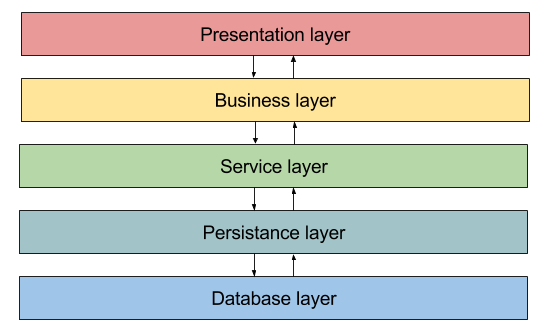
\includegraphics[scale=0.4]{img/LayeredArchitecture}
		\caption{Architettura a layer adottata nell'applicazione}
		\label{fig:LayerArchitecture}
	\end{figure}
		
	
	%\subsection{Componenti principali architettura}
		
		% Descrizione interazioni tra le componenti
		
		%include package no method

\end{document}